
% ! NEW code
\begin{tikzpicture}[scale=0.5]
    % Define the tiles
    \def\tileA{(0,0) rectangle (1,1)}
    \def\tileB{(1,0) rectangle (2,1)}
    
    % Draw the tiling pattern
    \foreach \x in {0,1,2,3}{
      \foreach \y in {0,1}{
        \draw \tileA (\x,\y);
        \draw \tileB (\x+0.5,\y+0.5);
      }
    }
  \end{tikzpicture}


% ! NEW code
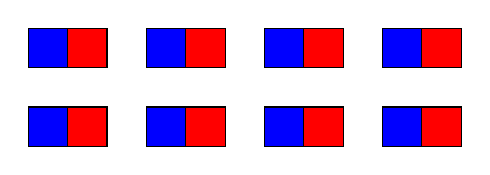
\begin{tikzpicture}[scale=0.5]
    % Define the tile
    \def\tile{
      % Insert TikZ commands for the tile here
      \draw[fill=blue] (0,0) rectangle (1,1);
      \draw[fill=red] (1,0) rectangle (2,1);
    }
    
    % Draw the tiling pattern
    \foreach \x in {0,1,2,3}{
      \foreach \y in {0,1}{
        \pgfmathsetmacro{\shiftX}{\x*3} % Set horizontal shift
        \pgfmathsetmacro{\shiftY}{\y*2} % Set vertical shift
        \begin{scope}[shift={(\shiftX,\shiftY)}]
          \tile
        \end{scope}
      }
    }
  \end{tikzpicture}

% ! NEW code
  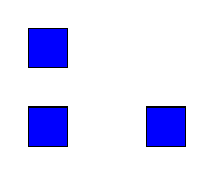
\begin{tikzpicture}[scale=0.5]
    % Define the tile
    \def\tile{
      % Insert TikZ commands for the tile here
      \draw[fill=blue] (0,0) rectangle (1,1);
      %\draw[fill=red] (1,0) rectangle (2,1);
    }
    
    % Draw the tiling pattern
    \tile % Draw the first tile at the origin
    \begin{scope}[shift={(3,0)}]
      \tile % Draw the second tile shifted three units to the right
    \end{scope}
    \begin{scope}[shift={(0,2)}]
      \tile % Draw the third tile shifted two units up
    \end{scope}
    % Continue adding more tiles with different shift values to create the desired tiling pattern
  \end{tikzpicture}


% ! NEW code
  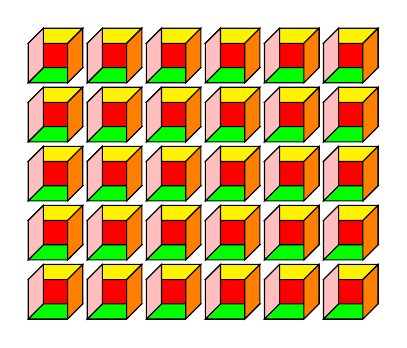
\begin{tikzpicture}[scale=0.5]
    % Define the tile
    \def\tile{
      % Draw the unit cube
      \draw[fill=blue] (0,0,0) -- (1,0,0) -- (1,1,0) -- (0,1,0) -- cycle;
      \draw[fill=red] (0,0,1) -- (1,0,1) -- (1,1,1) -- (0,1,1) -- cycle;
      \draw[fill=green] (0,0,0) -- (1,0,0) -- (1,0,1) -- (0,0,1) -- cycle;
      \draw[fill=yellow] (0,1,0) -- (1,1,0) -- (1,1,1) -- (0,1,1) -- cycle;
      \draw[fill=pink] (0,0,0) -- (0,1,0) -- (0,1,1) -- (0,0,1) -- cycle;
      \draw[fill=orange] (1,0,0) -- (1,1,0) -- (1,1,1) -- (1,0,1) -- cycle;
    }
  
    % Draw the tiling pattern
    \foreach \x in {0,1,2,3,4,5}{
      \foreach \y in {0,1,2,3,4}{
        \pgfmathsetmacro{\shiftX}{\x*1.5} % Set horizontal shift
        \pgfmathsetmacro{\shiftY}{\y*1.5} % Set vertical shift
        \begin{scope}[shift={(\shiftX,\shiftY,0)}]
          \tile % Draw the tile
        \end{scope}
      }
    }
  \end{tikzpicture}

  % ! NEW code
  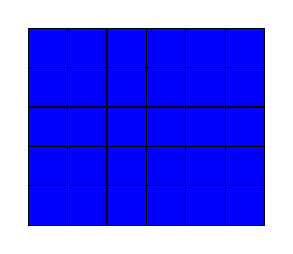
\begin{tikzpicture}[scale=0.5]
    % Define the tile
    \def\tile{
      % Draw the unit square with fill color
      \draw[fill=blue] (0,0) rectangle (1,1);
    }
  
    % Draw the tiling pattern
    \foreach \x in {0,1,2,3,4,5}{
      \foreach \y in {0,1,2,3,4}{
        \pgfmathsetmacro{\shiftX}{\x} % Set horizontal shift
        \pgfmathsetmacro{\shiftY}{\y} % Set vertical shift
        \begin{scope}[shift={(\shiftX,\shiftY)}]
          \tile % Draw the tile
        \end{scope}
      }
    }
  \end{tikzpicture}

% ! NEW code
  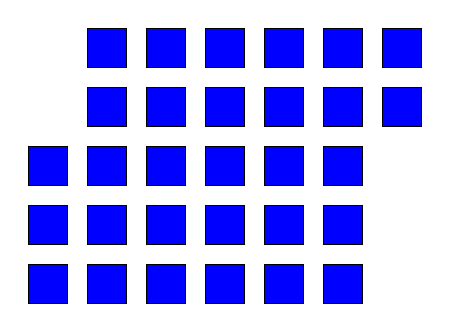
\begin{tikzpicture}[scale=0.5]
    % Define the tile
    \def\tile{
      % Draw the unit square with fill color
      \draw[fill=blue] (0,0) rectangle (1,1);
    }
  
    % Draw the tiling pattern
    \foreach \x in {0,1,2,3,4,5}{
      \foreach \y in {0,1,2,3,4}{
        \pgfmathsetmacro{\shiftX}{\x*1.5 + (1.5*\y > 3.5 ? 1.5 : 0)} % Set horizontal shift
        \pgfmathsetmacro{\shiftY}{\y*1.5} % Set vertical shift
        \begin{scope}[shift={(\shiftX,\shiftY)}]
          \tile % Draw the tile
        \end{scope}
      }
    }
  \end{tikzpicture}


% ! NEW code  
%? er denne firkantet
  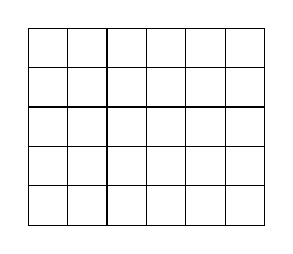
\begin{tikzpicture}[scale=0.5]
    % Define the tile
    \def\tile{
      % Draw the unit square
      \draw (0,0) rectangle (1,1);
    }
  
    % Draw the tiling pattern
    \foreach \x in {0,1,2,3,4,5}{
      \foreach \y in {0,1,2,3,4}{
        \pgfmathsetmacro{\shiftX}{\x} % Set horizontal shift
        \pgfmathsetmacro{\shiftY}{\y} % Set vertical shift
        \begin{scope}[shift={(\shiftX,\shiftY)}]
          \tile % Draw the tile
        \end{scope}
      }
    }
  \end{tikzpicture}

  % ! NEW code
  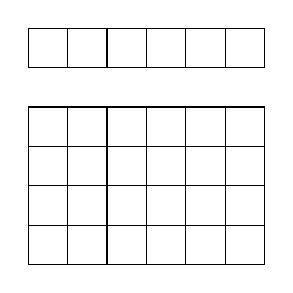
\begin{tikzpicture}[scale=0.5]
    % Define the tile
    \def\tile{
      % Draw the unit square
      \draw (0,0) rectangle (1,1);
    }
  
    % Draw the tiling pattern
    \foreach \x in {0,1,2,3,4,5}{
      \foreach \y in {0,1,2,3,4}{
        \pgfmathsetmacro{\shiftX}{\x} % Set horizontal shift
        \pgfmathsetmacro{\shiftY}{\y + (\y > 3.5 ? 1:0)} % Set vertical shift
        \begin{scope}[shift={(\shiftX,\shiftY)}]
          \tile % Draw the tile
        \end{scope}
      }
    }
  \end{tikzpicture}

% ! NEW code
  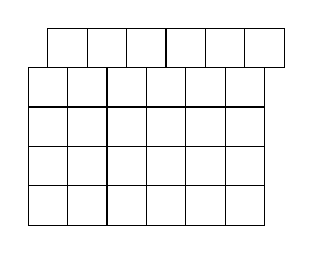
\begin{tikzpicture}[scale=0.5]
    % Define the tile
    \def\tile{
      % Draw the unit square
      \draw (0,0) rectangle (1,1);
    }
  
    % Draw the tiling pattern
    \foreach \x in {0,1,2,3,4,5}{
      \foreach \y in {0,1,2,3,4}{
        \pgfmathsetmacro{\shiftX}{\x + (\y > 3.5 ? 0.5 : 0)} % Set horizontal shift
        \pgfmathsetmacro{\shiftY}{\y} % Set vertical shift
        \begin{scope}[shift={(\shiftX,\shiftY)}]
          \tile % Draw the tile
        \end{scope}
      }
    }
  \end{tikzpicture}


% ! NEW code
  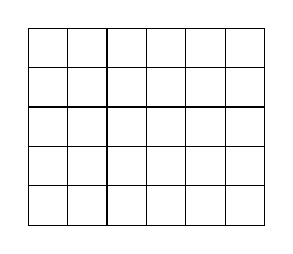
\begin{tikzpicture}[scale=0.5]
    % Define the tile
    \def\tile{
      % Draw the unit square
      \draw (0,0) rectangle (1,1);
    }
  
    % Draw the tiling pattern
    \foreach \x in {0,1,2,3,4,5}{
      \foreach \y in {0,1,2,3,4}{
        \pgfmathsetmacro{\shiftX}{\x} % Set horizontal shift
        \pgfmathsetmacro{\shiftY}{\y + (3.5 > \x > 2.5 ? 0.5 : 0)} % Set vertical shift
        \begin{scope}[shift={(\shiftX,\shiftY)}]
          \tile % Draw the tile
        \end{scope}
      }
    }
  \end{tikzpicture}

% ! NEW code
  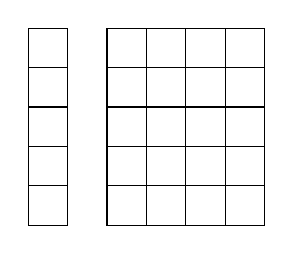
\begin{tikzpicture}[scale=0.5]
    % Define the tile
    \def\tile{
      % Draw the unit square
      \draw (0,0) rectangle (1,1);
    }
  
    % Draw the tiling pattern
    \foreach \x in {0,1,2,3,4,5}{
      \ifnum\x < 3
        \pgfmathsetmacro{\shiftX}{\x + (\x > 0 ? 1 : 0)} % Set horizontal shift
      \else
        \pgfmathsetmacro{\shiftX}{\x} % No horizontal shift for the last three columns
      \fi
      \foreach \y in {0,1,2,3,4}{
        \pgfmathsetmacro{\shiftY}{\y} % No vertical shift
        \begin{scope}[shift={(\shiftX,\shiftY)}]
          \tile % Draw the tile
        \end{scope}
      }
    }
  \end{tikzpicture}

% ! NEW code
  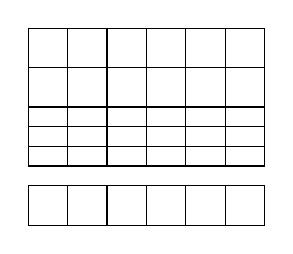
\begin{tikzpicture}[scale=0.5]
    % Define the tile
    \def\tile{
      % Draw the unit square
      \draw (0,0) rectangle (1,1);
    }
  
    % Draw the tiling pattern
    \foreach \x in {0,1,2,3,4,5}{
      \foreach \y in {0,1,2,3,4}{
        \pgfmathsetmacro{\shiftX}{\x} % No horizontal shift
        \ifnum\y<2
          \pgfmathsetmacro{\shiftY}{\y + (\y > 0 ? 0.5 : 0)} % Set vertical shift
        \else
          \pgfmathsetmacro{\shiftY}{\y} % No vertical shift for the last three rows
        \fi
        \begin{scope}[shift={(\shiftX,\shiftY)}]
          \tile % Draw the tile
        \end{scope}
      }
    }
  \end{tikzpicture}


% ! NEW code
  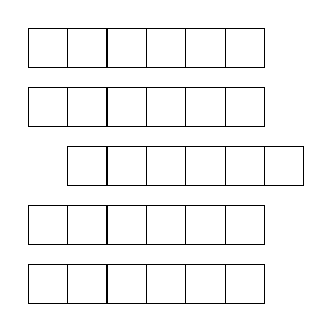
\begin{tikzpicture}[scale=0.5]
    % Define the tile
    \def\tile{
      % Draw the unit square
      \draw (0,0) rectangle (1,1);
    }
  
    % Draw the tiling pattern
    \foreach \x in {0,1,2,3,4,5}{
      \foreach \y in {0,1,2,3,4}{
        \ifnum\y=2 % Set horizontal shift for the third row only
          \pgfmathsetmacro{\shiftX}{\x + 1} % Shift one unit to the right
        \else
          \pgfmathsetmacro{\shiftX}{\x} % No horizontal shift for other rows
        \fi
        \pgfmathsetmacro{\shiftY}{\y} % No vertical shift
        \begin{scope}[shift={(\shiftX,\shiftY*1.5)}]
          \tile % Draw the tile
        \end{scope}
      }
    }
  \end{tikzpicture}


% ! NEW code 
%? DENNE VIL VI HA + linje 127
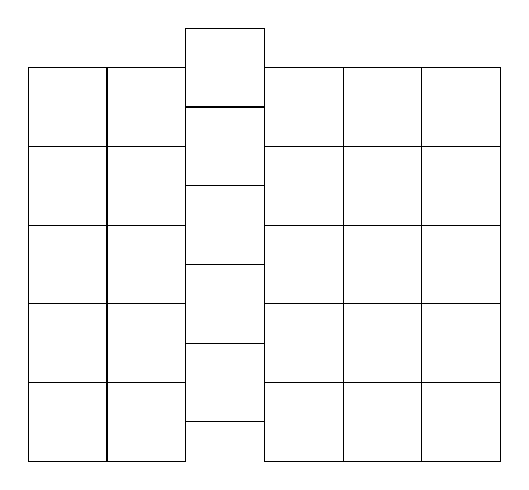
\begin{tikzpicture}[scale=1]
  % Define the tile
  \def\tile{
  % Draw the unit square
  \draw (0,0) rectangle (1,1);
  }

  % Draw the tiling pattern
  \foreach \x in {0,1,2,3,4,5}{
  \foreach \y in {0,1,2,3,4}{
      \ifnum\x=2 % Set vertical shift for the third column only
      \pgfmathsetmacro{\shiftX}{\x} % No vertical shift for other columns
      \pgfmathsetmacro{\shiftY}{\y + 0.5} % Shift one unit upward
      \else
      \pgfmathsetmacro{\shiftX}{\x} % No vertical shift for other columns
      \pgfmathsetmacro{\shiftY}{\y} % No vertical shift
      \fi
      \begin{scope}[shift={(\shiftX,\shiftY)}]
      \tile % Draw the tile
      \end{scope}
  }
  }
\end{tikzpicture}